\documentclass{beamer}
\usetheme{Madrid}
\usecolortheme{default}


\title[Target-Speaker STT]
{Target-Speaker Speech-to-Text\\in Overlapping Speech}

\subtitle{ECE1508 -- Applied Deep Learning}

\author[Shah \& Attafuah]
{Jibran Iqbal Shah \and Yamoah Frimpong Attafuah}

\institute[UofT]
{
  University of Toronto
}

\date[AplDL]
{ECE1508 -- Applied Deep Learning}

\logo{
\includegraphics[height=0.8cm]{logo_uoft}}

\definecolor{uoftblue}{RGB}{6,41,88}
\setbeamercolor{titlelike}{bg=uoftblue}
\setbeamerfont{title}{series=\bfseries}

\usepackage{booktabs}
\usepackage{graphicx}
% Smaller body text globally
\usepackage{tikz}
\usetikzlibrary{positioning, calc, arrows.meta}
\usetikzlibrary{positioning, calc, arrows.meta}
\setbeamerfont{normal text}{size=\small}
\setbeamerfont{itemize/enumerate body}{size=\small}
\setbeamerfont{block body}{size=\small}

\begin{document}

\begin{frame}
\vspace{0.3cm}
{\Large\bfseries\color{uoftblue} Target-Speaker Speech-to-Text in Overlapping Speech}

\vspace{0.1cm}
{\small Jibran Iqbal Shah \& Yamoah Frimpong Attafuah \hfill University of Toronto}

\vspace{0.3cm}

\small
\begin{itemize}
    \item Modern ASR systems like Whisper perform well on clean single-speaker audio
    \item But in meetings, courtrooms, and media, speakers frequently overlap
    \item Standard ASR tries to transcribe every voice together, which causes errors
\end{itemize}

\vspace{0.15cm}

\textbf{Goal:} Given a multi-speaker audio mixture and a short enrollment clip, transcribe only the target speaker.

\vspace{0.15cm}

\begin{block}{Why does this matter?}
\small
Accurate per-speaker transcription is needed in courtrooms, podcasts, debates, and meetings. It also enables labelling data for full-duplex speech models.
\end{block}

\end{frame}


%% SLIDE 2: Whisper architecture + fine-tuning
\begin{frame}
\frametitle{Our ASR Model: Whisper}

\small

We use OpenAI's Whisper as our ASR backbone. Whisper is a transformer-based encoder-decoder model trained on 680{,}000 hours of multilingual speech.

\vspace{0.2cm}

\centering
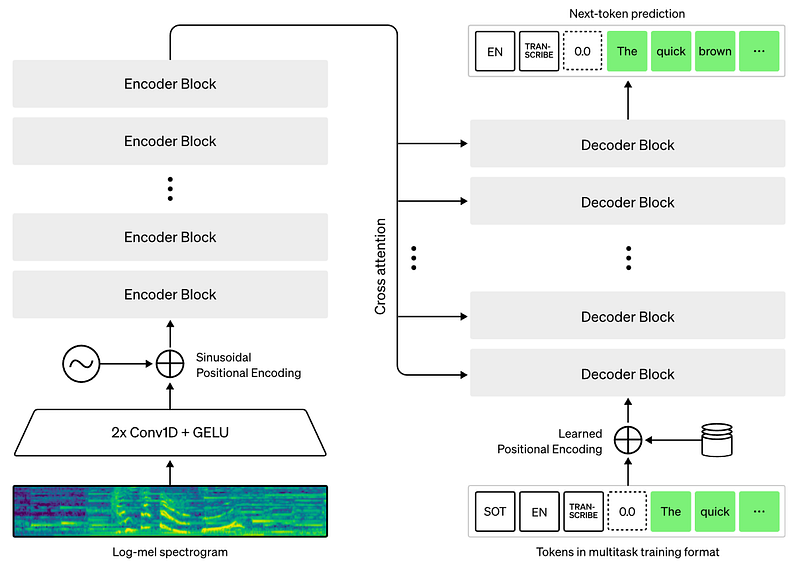
\includegraphics[height=0.42\textheight]{whispermodel.png}

\vspace{0.3cm}

\flushleft
\small
\begin{itemize}
    \item English: We use Whisper-tiny (39M params) off the shelf
    \item Twi (Akan): Whisper does not support Twi natively, so we fine-tuned Whisper-small (244M params) on the WAXAL Akan dataset
    \item Both models serve as baselines to measure how overlap degrades transcription and whether the trend is observed across languages
\end{itemize}

\end{frame}


%% SLIDE 3: Results -- English + Twi side by side
\begin{frame}
\frametitle{Overlap Degrades ASR Across Languages}

\small
12{,}500 synthetic two-speaker mixtures per language ($\mathbf{x}_{\text{mix}} = \mathbf{x}_{\text{target}} + \alpha\,\mathbf{x}_{\text{interferer}}$) at varying SIR levels and overlap ratios.

\vspace{0.1cm}

\begin{columns}[T]
\begin{column}{0.48\textwidth}
    \centering
    \scriptsize English (Whisper-tiny)
    
\includegraphics[width=\textwidth]{English_Base_Whisper_WER_vs_Overlap.png}
\end{column}
\begin{column}{0.48\textwidth}
    \centering
    \scriptsize Twi (fine-tuned Whisper-small)
    
\includegraphics[width=\textwidth]{Twi_Finetuned_Whisper_WER_vs_Overlap.png}
\end{column}
\end{columns}

\vspace{0.1cm}

\small
\begin{itemize}
    \item English clean baseline: 8.1\% WER. At 0\,dB SIR with full overlap, WER exceeds 100\%.
    \item Twi clean baseline: 34.7\% WER. Same degradation pattern.
    \item This problem is language agnostic.
\end{itemize}

\end{frame}


%% SLIDE 4: Our approach + what's next
\begin{frame}
\frametitle{Proposed Solution: Speaker-Conditioned Masking}

\small
The mixture waveform is converted to a magnitude spectrogram $|\mathbf{X}_{\text{mix}}| \in \mathbb{R}^{F \times T}$ via the Short-Time Fourier Transform, where each entry represents the energy at a given frequency and time frame. 

\vspace{0.6mm}
We predict a soft mask $\mathbf{M} \in [0,1]^{F \times T}$, conditioned on a speaker embedding $\mathbf{e}$ from a frozen pretrained speaker verification model.

\vspace{0.15cm}

\begin{center}
\scalebox{0.85}{%
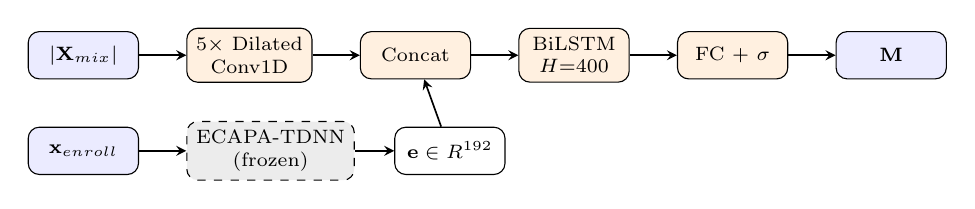
\begin{tikzpicture}[
    node distance=0.4cm and 0.6cm,
    box/.style={draw, rounded corners, minimum height=0.6cm, minimum width=1.4cm, align=center, font=\scriptsize},
    io/.style={box, fill=blue!8},
    op/.style={box, fill=orange!12},
    frozen/.style={box, fill=gray!15, dashed},
    arr/.style={-stealth, semithick},
]
\node[io] (mag) {$|\mathbf{X}_{\text{mix}}|$};
\node[io, below=0.6cm of mag] (enroll) {$\mathbf{x}_{\text{enroll}}$};
\node[frozen, right=0.6cm of enroll] (ecapa) {ECAPA-TDNN\\(frozen)};
\draw[arr] (enroll) -- (ecapa);
\node[box, right=0.5cm of ecapa] (emb) {$\mathbf{e} \in \mathbb{R}^{192}$};
\draw[arr] (ecapa) -- (emb);
\node[op, right=0.6cm of mag] (cnn) {5$\times$ Dilated\\Conv1D};
\draw[arr] (mag) -- (cnn);
\node[op, right=0.6cm of cnn] (concat) {Concat};
\draw[arr] (cnn) -- (concat);
\draw[arr] (emb) -- (concat);
\node[op, right=0.6cm of concat] (bilstm) {BiLSTM\\$H{=}400$};
\draw[arr] (concat) -- (bilstm);
\node[op, right=0.6cm of bilstm] (fc) {FC + $\sigma$};
\draw[arr] (bilstm) -- (fc);
\node[io, right=0.6cm of fc] (mask) {$\mathbf{M}$};
\draw[arr] (fc) -- (mask);
\end{tikzpicture}
}%
\end{center}

\vspace{0.1cm}

The predicted mask is applied to the mixture spectrogram $|\hat{\mathbf{X}}_{\text{target}}| = \mathbf{M} \odot |\mathbf{X}_{\text{mix}}|$ to reconstruct the target speaker's waveform, and Whisper does ASR on that.

\vspace{0.15cm}

Training loss (MSE between masked mixture and clean target spectrogram):
\[
    \mathcal{L} = \frac{1}{FT} \bigl\| \mathbf{M} \odot |\mathbf{X}_{\text{mix}}| - |\mathbf{X}_{\text{target}}| \bigr\|_F^2
\]

\end{frame}


%% SLIDE 5: Early results and next steps
\begin{frame}
\frametitle{Early Results and Next Steps}

\small
For now, the training loss isn't really going down from init, and we are slowly making the model more complex/larger.

With the best model so far, WER drops from 103.7\% without extraction to 78.5\% with extraction, which is a 24\% relative improvement on the hardest case, but there isn't a signficant difference on the smaller overlaps. 

\vspace{0.15cm}

\textbf{Current issues:} Training loss plateaus early and does not decrease significantly, suggesting the model may need higher capacity or better regularization or better training data to generalize better. 

\vspace{0.15cm}

\textbf{Next steps:}
\begin{itemize}
    \item Train only on data with $\geq 50\%$ overlap and add dropout
    \item Try out other architectures (more conv layers? larger embedding dimension? Transformer?)
    \item Ablations: enrollment clip length, SIR sensitivity
    \item Cross-lingual transfer: train on English, test on Twi
\end{itemize}

\end{frame}

\end{document}